\documentclass{article}
\usepackage{amsmath}
\usepackage{graphicx}
\usepackage{float}

\title{Is Batting Average Overrated?}
\author{Gabriel DeSouza}
\date{June 17, 2026}

\begin{document}

\maketitle

\tableofcontents
\newpage

\section{Introduction}

\hspace{12pt} Batting average is one of the most recognizable statistics in baseball. It is commonly displayed during broadcasts, alongside player names in 
scorebugs and lineup graphics, and has long been used as a measure of offensive performace. For many fans, batting average is often the first statistic considered 
when evaluating a hitter. 

\vspace{5pt}

Despite its popularity, the value of batting average has become heavily debated in recent decades. Many analysts argue that metrics like on-base percentage (OBP)
, slugging percentage (SLG), and on-base plus slugging (OPS) offer more accurate indicators of offensive contribution due to the growth of sabermetrics and 
advanced baseball analytics. Unlike batting average, these statistics account for factors such as walks and extra-base hits, which may have a greater impact on a team's ability to score runs 
and win games.

\vspace{5pt}

As a result, an important question emerges: 

\vspace{2pt}

\textbf{Is batting average still a meaningful indicator of team success, or have modern offensive metrics replaced its
 usefulness?}

\vspace{5pt}

The goal of this project is to investigate the relationships between several offensive statistics and runs scored in the MLB since 2000. Particular 
attention is given to batting average, on-base percentage, slugging percentage, OPS, walk rate, strikeout rate, and isolated power. By comparing the strength of 
the relationships between these statistics and runs scored, this analysis seeks to whether batting average remains a valuable measure of team success compared to 
more modern metrics.

\vspace{20pt}

\section{Data Description}

\hspace{12pt} The data used in this analysis were obtained from the Lahman Baseball Database, a publicly available collection of historical Major League Baseball 
statistics. The original dataset contains team-level records spanning more than a century of professional baseball history. To focus on the modern era of the 
sport, only observations from the 2000 season onward were retained. Additionally, the 2020 season was excluded from the analysis due to its shortened 60-game 
schedule resulting from the COVID-19 pandemic.

\vspace{5pt}

Each observation in the dataset represents a single Major League Baseball team during a particular season. After filtering, the dataset contained 750 team-seasons. 
Several offensive variables were selected for analysis, including at-bats (AB), hits (H), doubles (2B), triples (3B), home runs (HR), walks (BB), strikeouts (SO), 
sacrifice flies (SF), and runs scored. 

\vspace{5pt}

Using these variables, several commonly used offensive statistics were calculated. Batting average (AVG) was included as a traditional measure of hitting 
performance, while on-base percentage (OBP), slugging percentage (SLG), and on-base plus slugging (OPS) were included as more comprehensive measures of offensive 
production. In addition, walk rate, strikeout rate, and isolated power (ISO) were calculated to display different aspects of offensive approach and effectiveness.

\vspace{5pt}

Before doing any statistical analysis, the dataset was examined for missing values and inconsistencies. No missing observations were found among the variables used 
in the study.

\vspace{20pt}

\section{Methods}

\hspace{12pt} To evaluate the relationships between offensive performance metrics and regular season success, a correlation-based approach was used. 

\vspace{5pt}

First, several offensive statistics were calculated from the raw team batting data. This includes: 

\vspace{5pt}

Batting Average: $avg = \frac{H}{AB}$ 

\vspace{5pt}

On-base Percentage: $obp = \frac{H + BB + HBP}{AB + BB + HBP + SF}$

\vspace{5pt}

Total Bases: $TB = H + 2B + 2*(3B) + 3*(HR)$

\vspace{5pt}

Slugging Percentage: $slg = \frac{TB}{AB}$

\vspace{5pt}

On-Base Plus Slugging: $ops = obp + slg$

\vspace{5pt}

Walk rate and Strikeout Rate: $\frac{BB}{PA}$ and $\frac{SO}{PA}$

\vspace{5pt}

Isolated Power: $iso = slg - avg$

\vspace{10pt}

These statistics were chosen because they represent different aspects of offensive performance, including a team's ability to generate hits, reach base, hit for 
power, draw walks, and avoid strikeouts.

\vspace{5pt}

Pearson correlation coefficients were then calculated between runs scored and each offensive statistic. The Pearson correlation coefficient provides a 
measure of the strength and direction of a linear relationship between two variables, taking values between -1 and 1. Values close to 1 indicate a strong positive 
association, values close to -1 indicate a strong negative association, and values near 0 suggest little or no linear relationship.

\vspace{5pt}

After calculating the correlation coefficients, the offensive statistics exhibiting the strongest relationships with runs were identified. Particular attention was 
given to comparing batting average with more modern offensive metrics such as OBP, SLG, and OPS. This comparison was motivated by the ongoing debate within 
baseball analytics regarding the usefulness of batting average as a measure of offensive performance.

\vspace{5pt}

To complement the numerical analysis, scatterplots were created to visualize the relationships between selected offensive statistics and runs scored. 
These visualizations were used to identify overall trends and compare the strength of relationships.

\vspace{20pt}

\section{Results}

\subsection{Batting Average}

\hspace{12pt} The first metric result I want to show is the main topic of the video: Batting Average. For those who don't know, batting average measures how many 
hits a player gets per at-bat.

\begin{figure}[H]
    \centering
    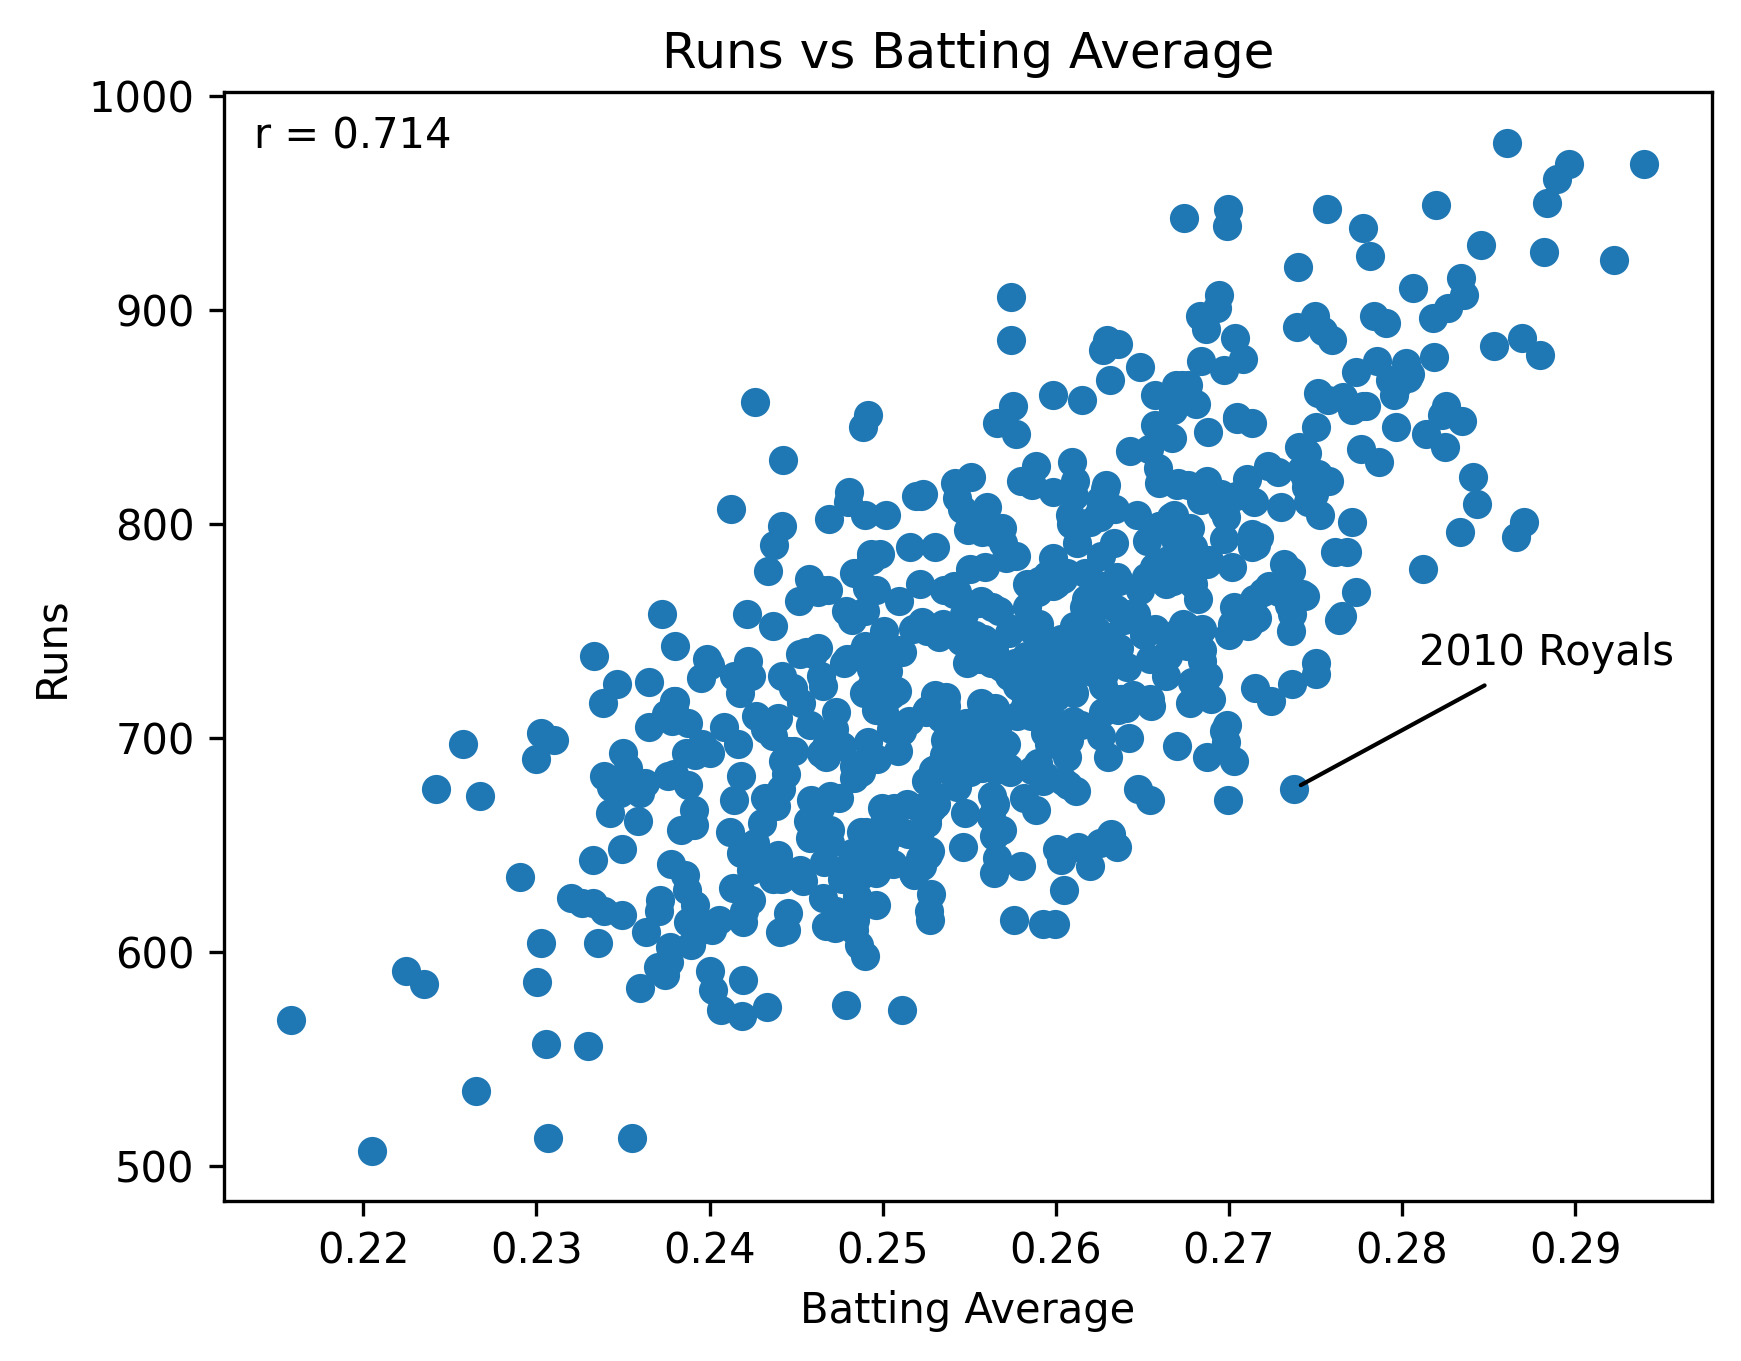
\includegraphics[width=0.8\textwidth]{runs_avg.png}
    \caption{Relationship between batting average and runs scored.}
    \label{fig:avg}
\end{figure}

Observing the graph, there is a somewhat strong linear relationship between batting average and runs. The relatively middling r-value of 0.714 
suggests this, along with a large amount of teams that prove to be great examples of why batting average alone is not a very accurate measure of success in the MLB.

\vspace{5pt}

A great example of this is the 2010 Royals, a team that batted above average with 0.274 but only ended up scoring 676 runs, with a record of 67-95.

\subsection{Metric Comparison}

Here's how every other metric analyzed compares to batting average in terms of correlation with runs. This chart makes it clear that the correlation between batting 
average and runs is not nearly as strong as other modern metrics.

\begin{figure}[H]
    \centering
    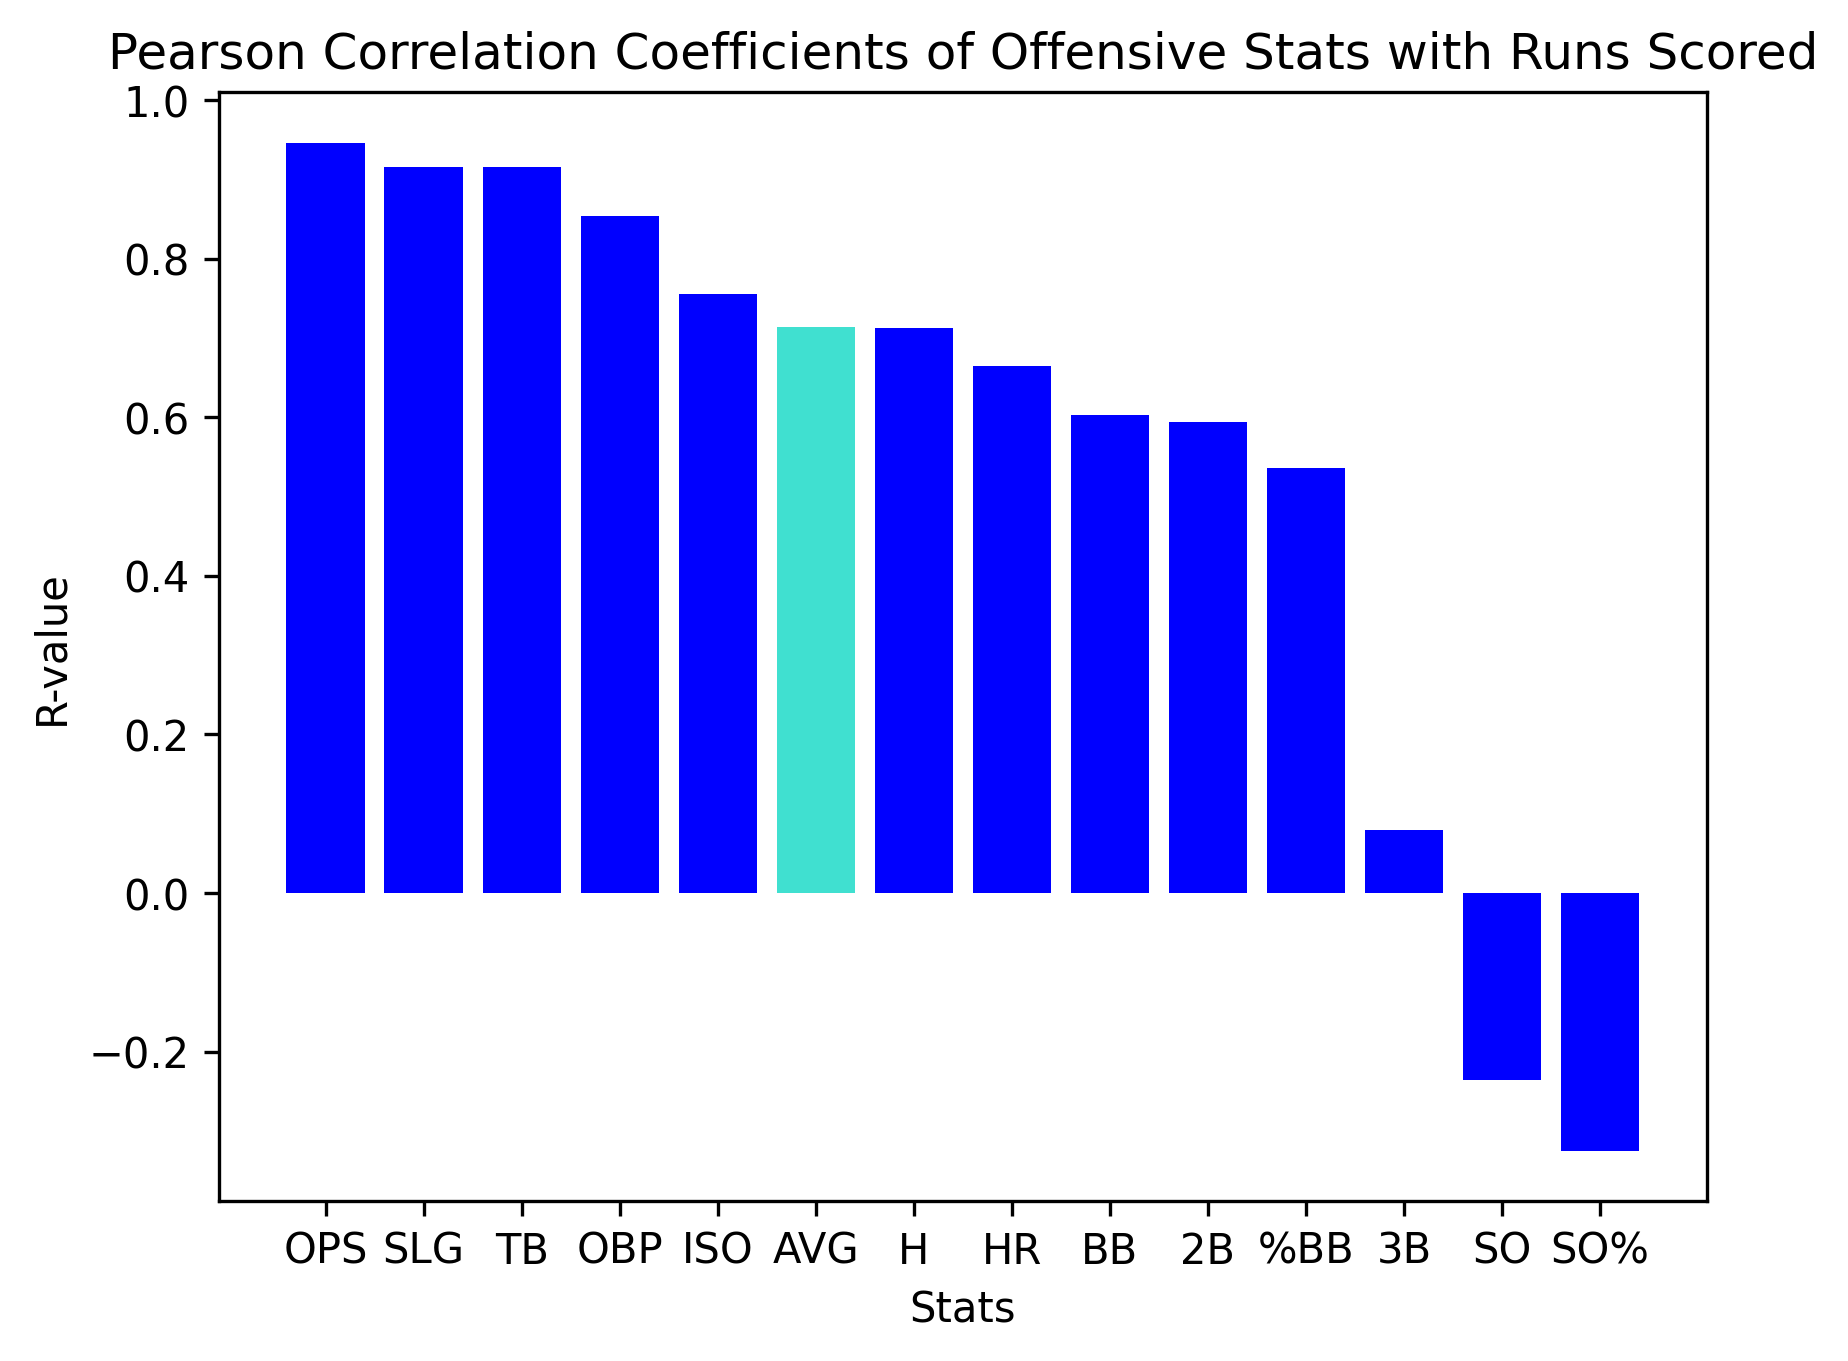
\includegraphics[width=0.8\textwidth]{rvalue_avg.png}
    \caption{R-values for each offensive metric analyzed.}
    \label{fig:ravg}
\end{figure}

\newpage

Let's look at the metrics that have the top 3 strongest correlations with runs.

\subsection{On-Base Percentage}

In 3rd place, we have On-Base Percentage. This is a very simple metric, measuring how often a player gets on base per 
plate appearance, hence the name on-base percentage.

\begin{figure}[H]
    \centering
    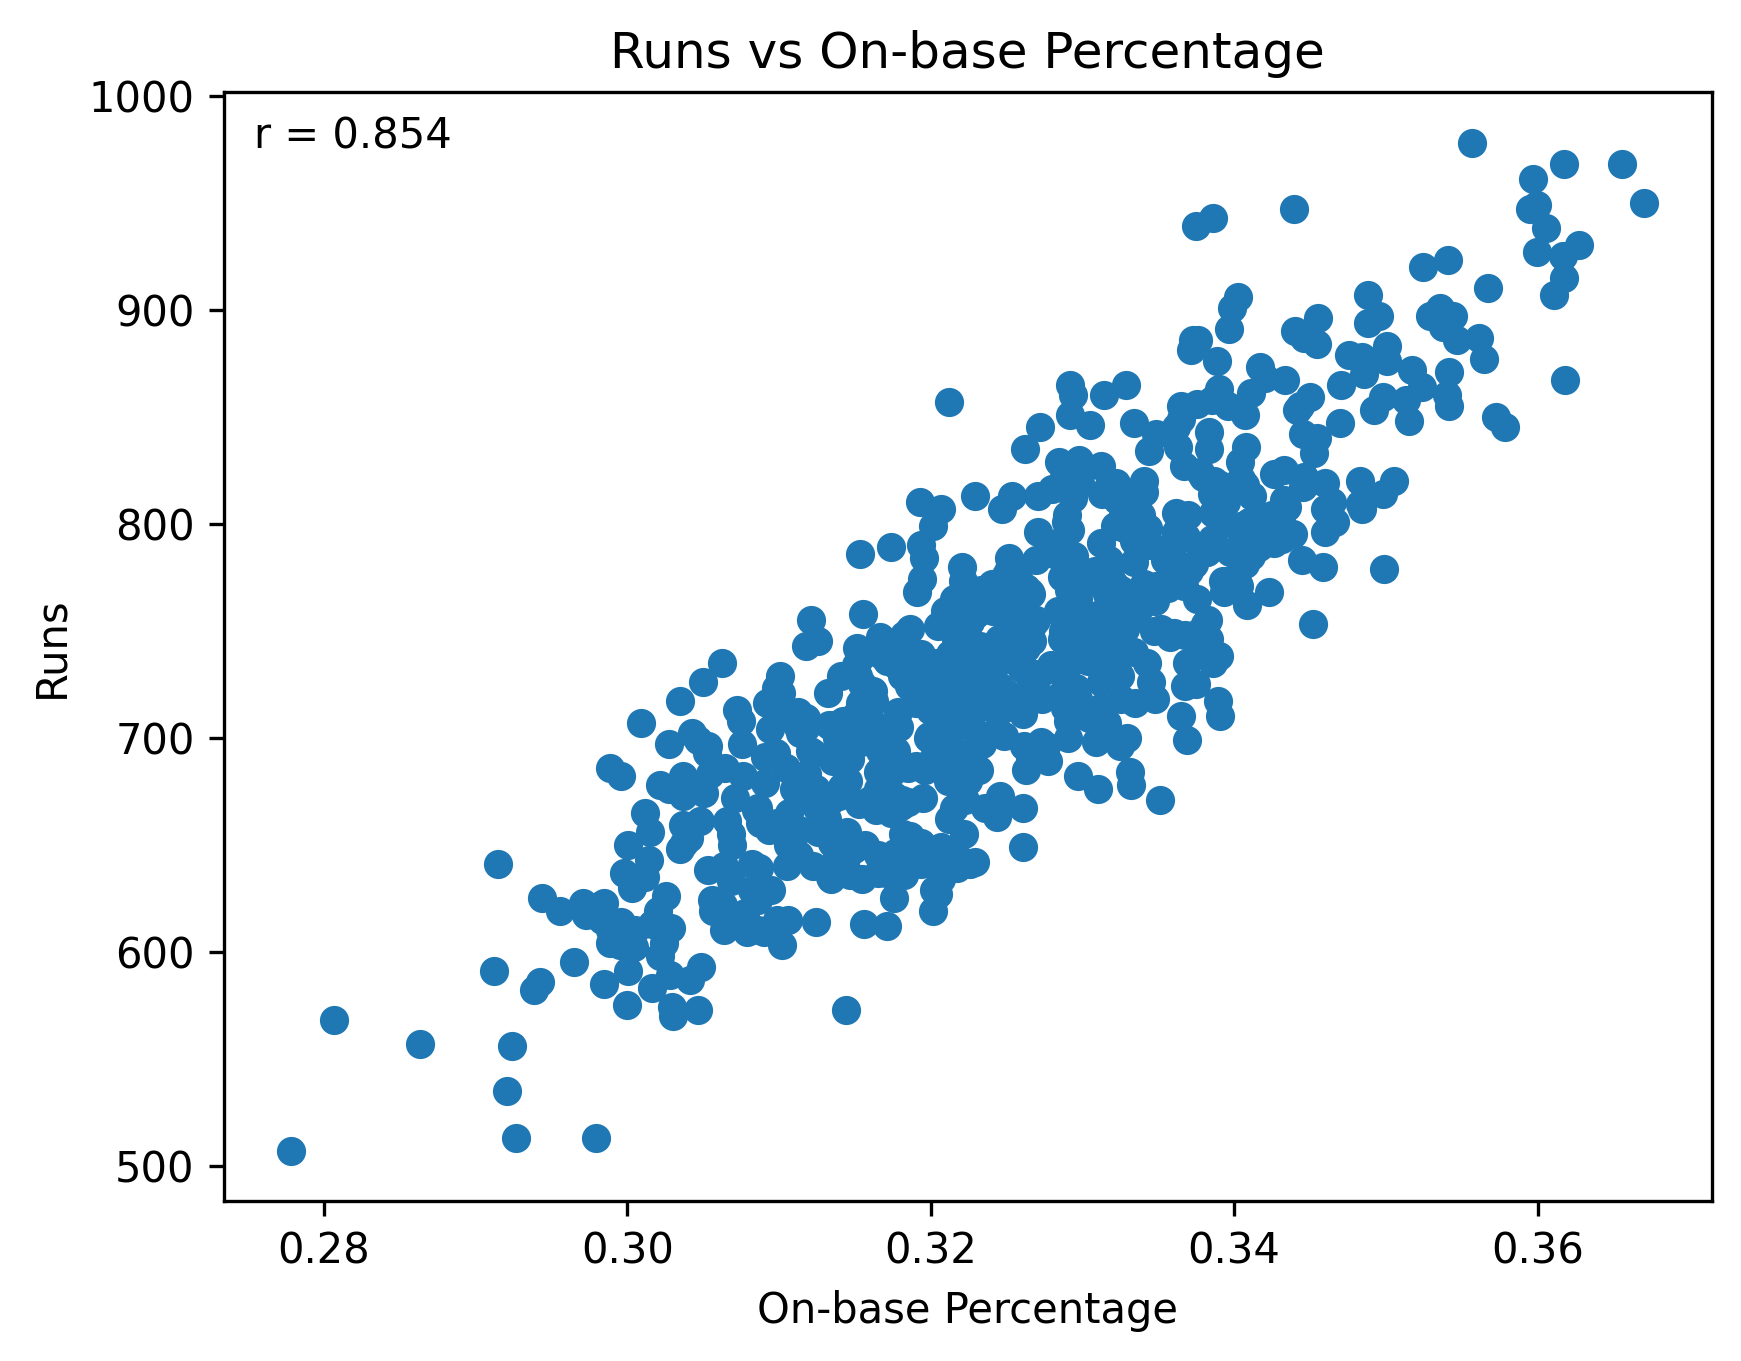
\includegraphics[width=0.8\textwidth]{runs_obp.png}
    \caption{Relationship between on-base percentage and runs scored.}
    \label{fig:obp}
\end{figure}

\vspace{10pt}

\newpage

\subsection{Slugging Percentage}

In 2nd place we have slugging percentage. Slugging Percentage is actually very similar to Batting Average, with one small difference. Slugging Percentage also measures how many hits a player gets per at 
bat, but weighs doubles, triples, and home runs increasingly heavier. This could be interpreted as a 'bases per at-bat' as opposed to hits per at bat.

\begin{figure}[H]
    \centering
    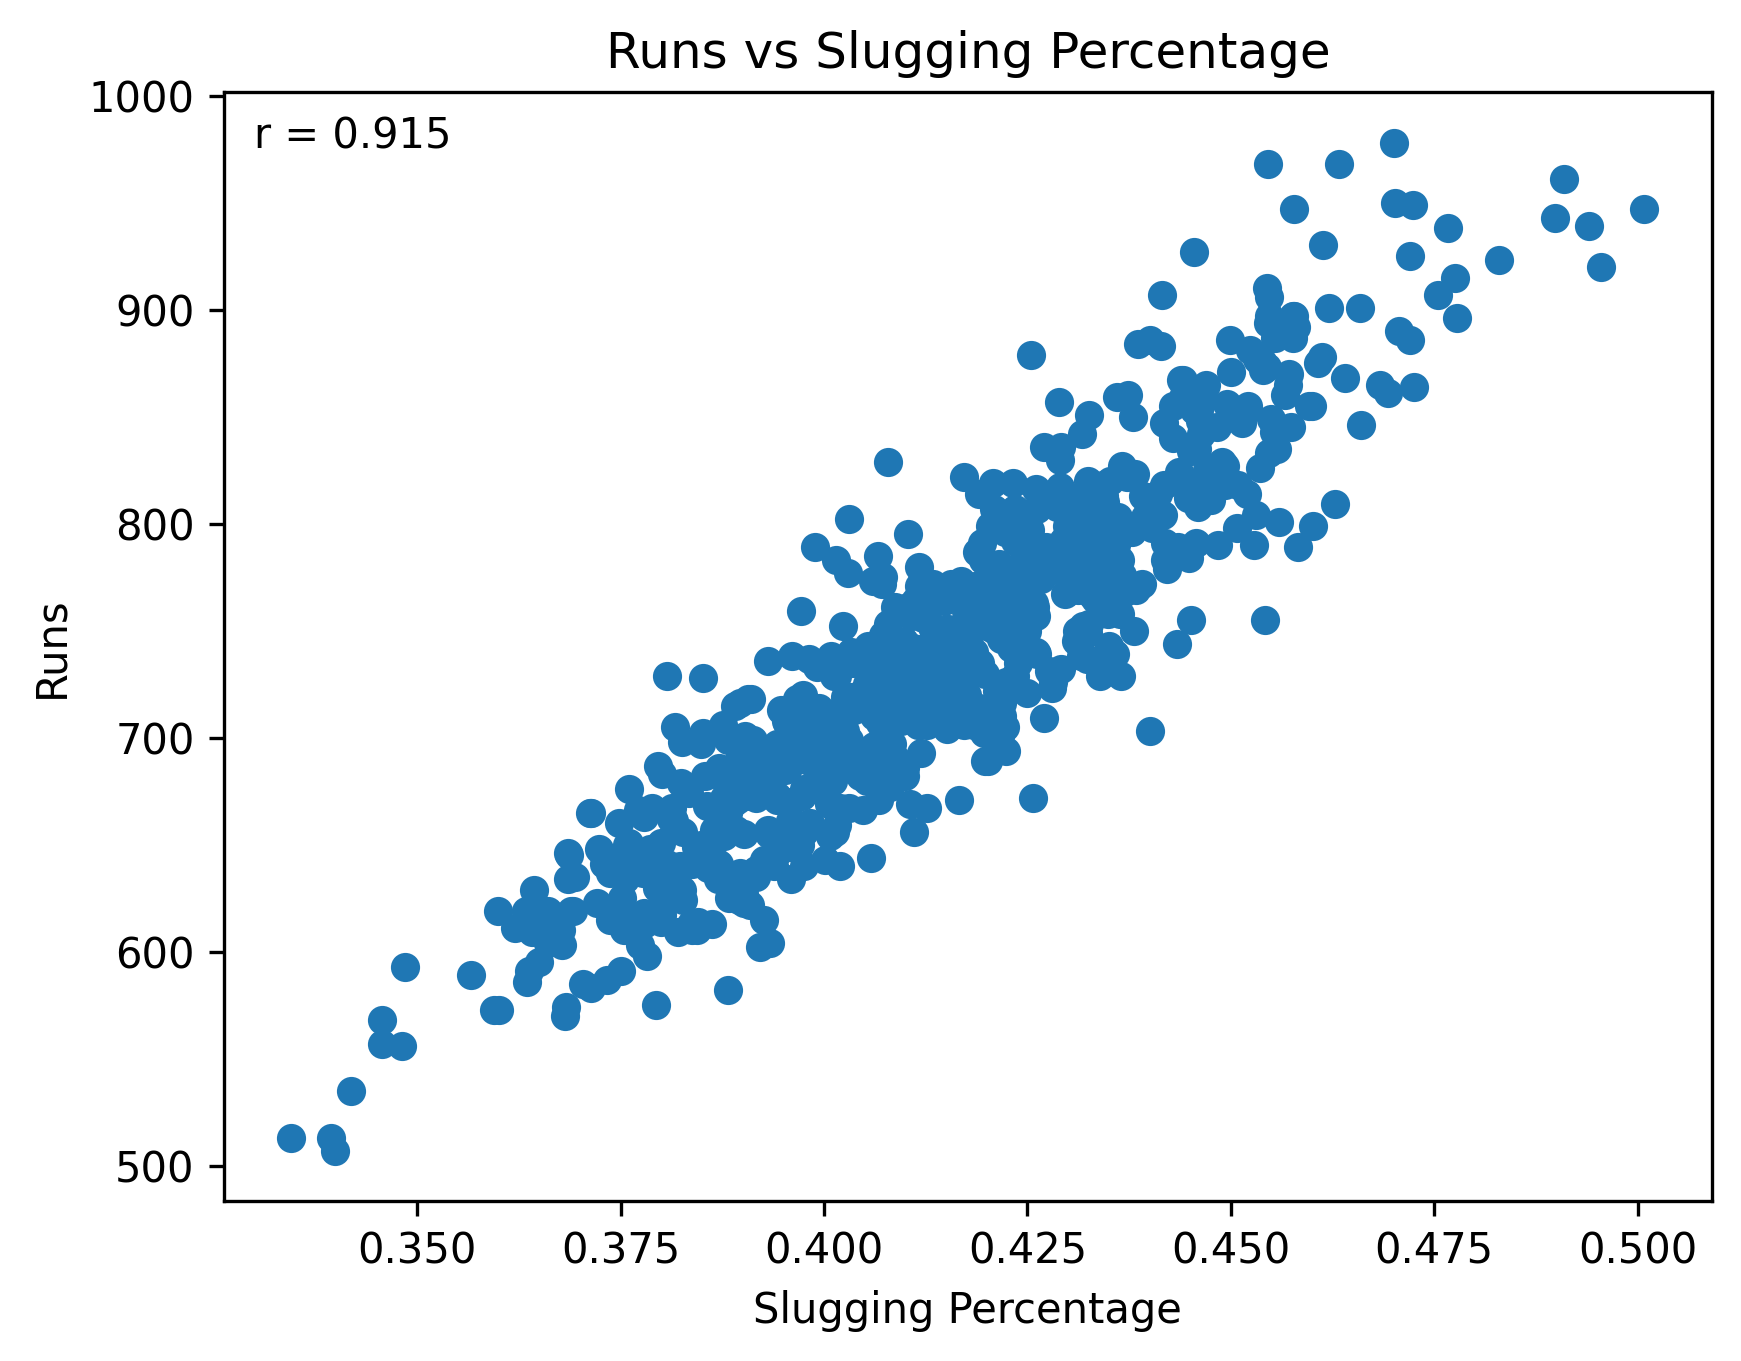
\includegraphics[width=0.8\textwidth]{runs_slg.png}
    \caption{Relationship between slugging percentage and runs scored.}
    \label{fig:slg}
\end{figure}

The visual makes it very clear that slugging has a much stronger correlation with runs than batting average.

\newpage

\subsection{OPS}

In 1st place is OPS. This metric simply adds the last two stats together, OBP and SLG.

\begin{figure}[H]
    \centering
    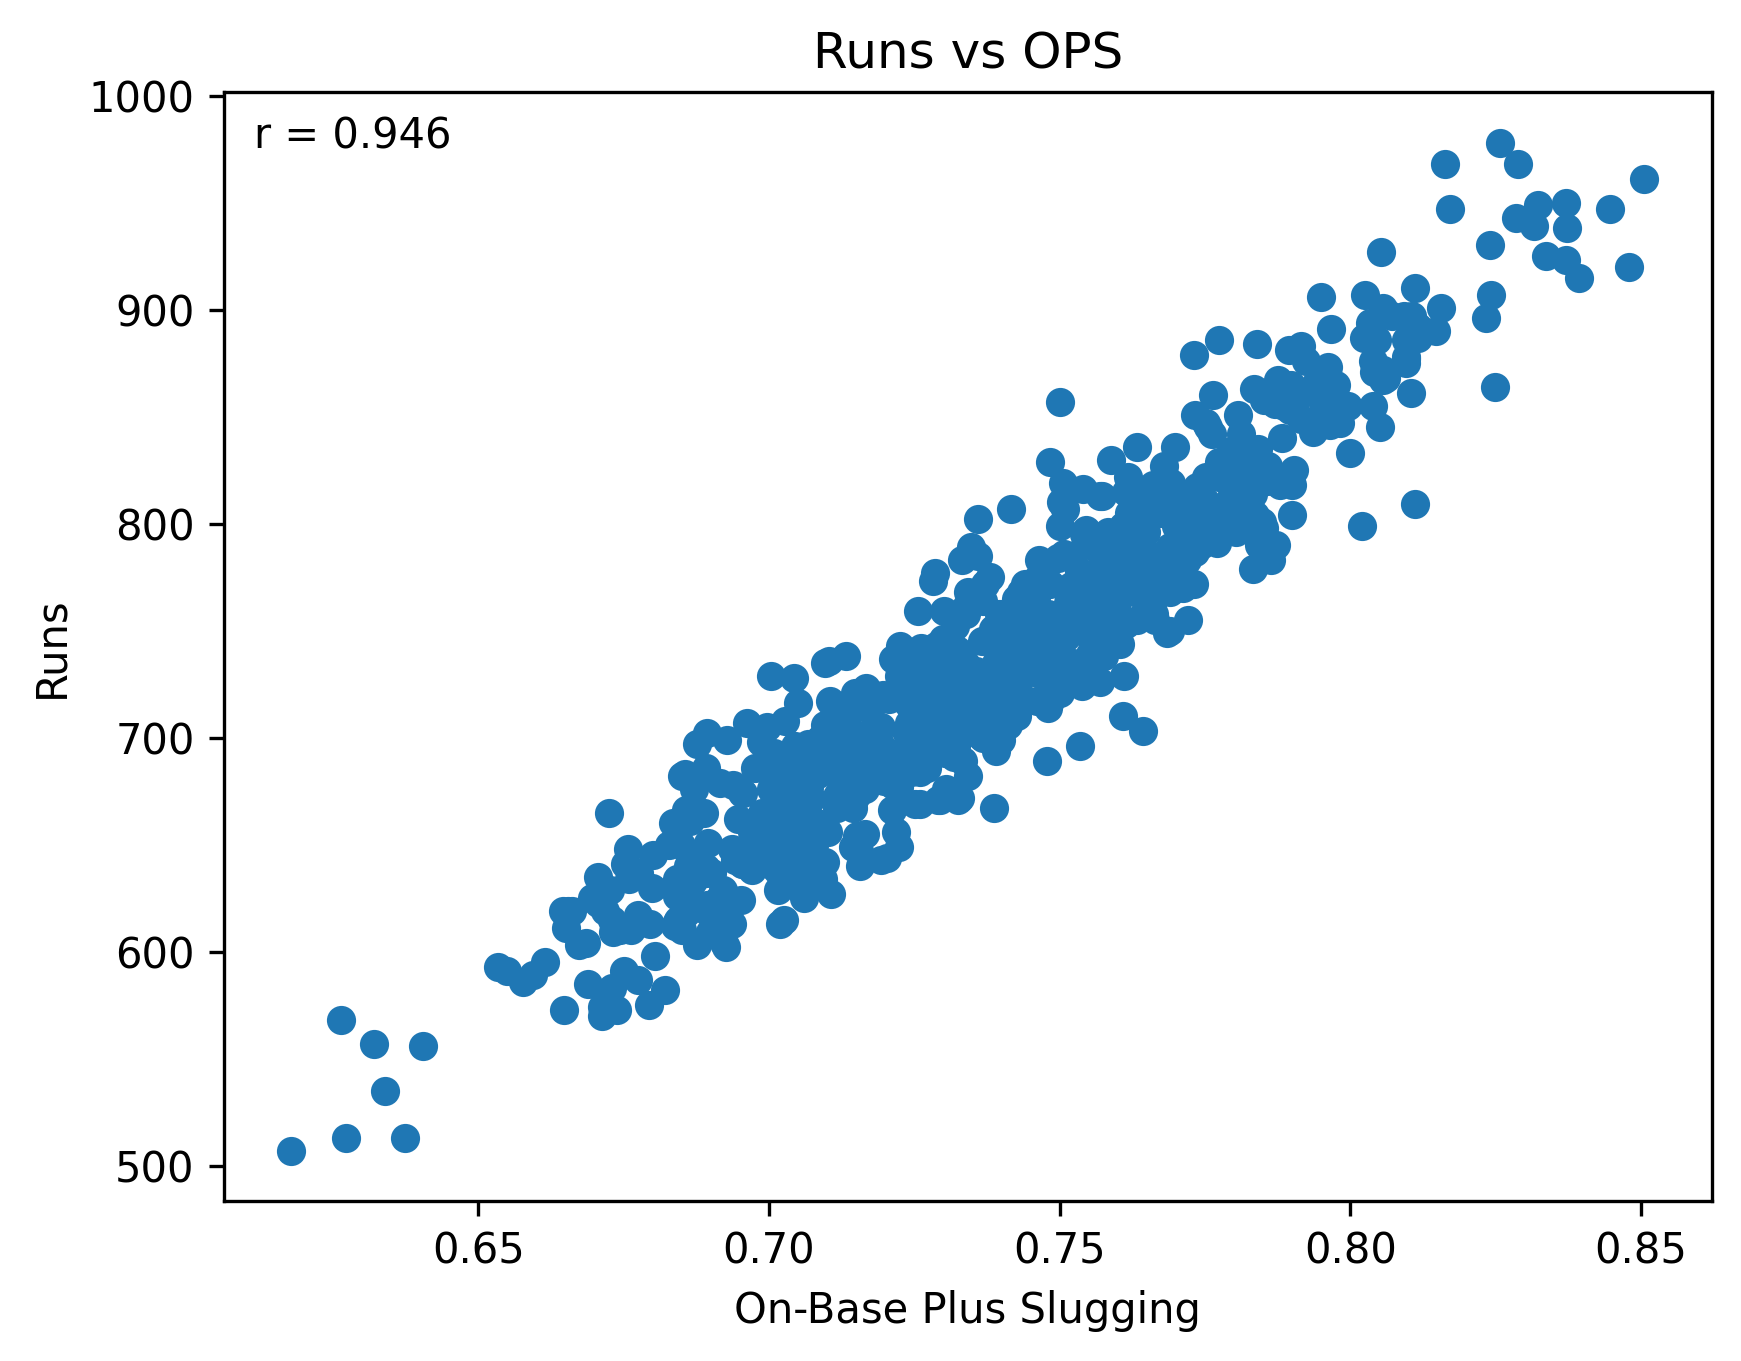
\includegraphics[width=0.8\textwidth]{runs_ops.png}
    \caption{Relationship between OPS and runs scored.}
    \label{fig:ops}
\end{figure}

\vspace{20pt}

\section{Discussion}

\hspace{12pt} The results of this analysis suggest that batting average is not nearly as strong of an indicator of team success as other modern metrics such as SLG, 
OBP and OPS. This supports the idea that simply recording hits is less informative than measuring the quality of those hits and a team's ability to generate total 
offensive production.

\vspace{5pt}

In particular, slugging percentage shows a noticeably stronger correlation with runs than batting average. This is because SLG accounts for extra-base hits, which 
contribute more directly to run scoring than singles. As a result, SLG better captures offensive power, which has a greater impact on a team's ability to win games.

\vspace{5pt}

On-base percentage performs even better than slugging in this analysis, highlighting the importance of avoiding outs. Since OBP includes hits, walks, and 
hit-by-pitches, it reflects a team's ability to sustain innings and create more scoring opportunities, which translates more directly into runs and wins.

\vspace{5pt}

OPS, which combines OBP and SLG, shows the strongest overall relationship with runs among the metrics tested. This suggests that a balanced measure of both 
getting on base and hitting for power provides a more complete representation of offensive value than any single component alone.

\vspace{5pt}

Overall, the results suggest that while batting average remains a familiar and widely used statistic, it is less informative than more modern offensive metrics. 
Measures that incorporate power and on-base ability provide a clearer connection to run production and team success in the modern era of baseball.

\vspace{20pt}

\section{Conclusion}

\hspace{12pt} This analysis shows that batting average is a relatively weak indicator of team success compared to more modern offensive metrics. While it remains a 
well-known and widely used statistic, it does not capture important aspects of offensive production such as power hitting or a team's ability to avoid making outs.

\vspace{5pt}

Metrics such as slugging percentage, on-base percentage, and especially OPS show stronger correlations with runs scored, suggesting that overall offensive 
value is better represented by a combination of getting on base and hitting for extra bases rather than simply recording hits.

\vspace{5pt}

Overall, the results back up the trend in baseball analytics toward more detailed measures of player and team value by supporting the idea that modern era 
sabermetric statistics give a more accurate understanding of offensive performance than traditional batting average.


\end{document}